%Commandi utili ridefiniti

\newcommand{\COURSE}{Ingegneria del software}

\newcommand{\STUDENT}{Grigoras Valentin}
\newcommand{\MATRICOLA}{1099561}
\newcommand{\ANNO}{A.A 2018/2019}




% ----------------------- TODO ---------------------------

\documentclass[a4paper]{article}
\usepackage[utf8]{inputenc}
\usepackage[T1]{fontenc}

\usepackage[italian]{babel}

\usepackage{fancyhdr}
\usepackage{color}

\usepackage{lastpage}
\usepackage{listings}
\usepackage{tikz}

\usepackage{subfigure}
\usepackage{float}
\usepackage{hyperref}
\usepackage{tabularx}
\usepackage{color}
\usepackage{geometry}
\usepackage{fancybox}

\usepackage{utopia}
\usepackage{lipsum}
\usepackage{amstext}
\usepackage{xcolor}
\usepackage{listingsutf8}
\lstset{inputencoding=utf8/latin1}
\definecolor{blue}{HTML}{007af7}
\definecolor{red}{HTML}{920022}
\definecolor{grey}{HTML}{fdfcf8}
\definecolor{comment}{HTML}{1b9852}
\definecolor{strings}{HTML}{5f283e}

\definecolor{tipo}{RGB}{167, 63, 74}
\definecolor{variabile}{RGB}{32, 114, 154}

\lstset{language=Java,backgroundcolor=\color{grey}, commentstyle=\color{comment},identifierstyle  = \color{blue},extendedchars=true, frame=single,keepspaces=true, keywordstyle=\color{red},tabsize=3,showstringspaces=false,literate={é}{{\'{e}}}1, literate={è}{{\'{e}}}1 }


\input kvmacros

%Größe der Ränder setzen
\geometry{a4paper,left=3cm, right=3cm, top=3cm, bottom=3cm}

%Kopf- und Fußzeile
\pagestyle {fancy}
\fancyhead[L]{\COURSE}
\fancyhead[C]{}
\fancyhead[R]{\rightmark }

\fancyfoot[L]{}
\fancyfoot[C]{}
\fancyfoot[R]{Pagina \thepage /\pageref*{LastPage}}

%Formatierung der Überschrift, hier nichts ändern
\def\header#1#2#3#4{
\vspace*{\fill}
  \begin{center}
    { \Large Appunti Ingegneria del software #1}\\ \vspace{10pt}
    {(\ANNO #2)} \\  \vspace{10pt}
{\Large \STUDENT#3} \\  \vspace{10pt}
{\Large Matricola: \MATRICOLA #4} \\  \vspace{10pt}
  \end{center}
  \vspace*{\fill}
}


\begin{document}

\header{}{}{}{}

\pagebreak

	\renewcommand{\contentsname}{Contenuti}
	\renewcommand\tablename{new}
	\tableofcontents \pagebreak

\vspace{30pt}
\section{Indicare le differenze (natura, finalita, collocazione) che intercorrono tra le attivitaa di \textbf{verifica} e quelle di \textbf{validazione}}
\subsection{Fissando l'attenzione sulla definizione di "processo" associata allo standard ISO/IEC 12207, indicare come (secondo quali regole), quando (in quali fasi di progetto) e perché (attraverso quali attività) la vostra esperienza di progetto didattico ha visto attuato tale concetto.}

Un processo è un insieme di attività \textbf{correlate}(ovvero contiene solo attività che hanno a che fare con il progetto)  e \textbf{coese}(un insieme di cose è coeso se tutto ciò che c’è serve, ci deve essere e se non ci fosse mancherebbe, quindi non c'è nulla di superfluo) con l'obiettivo di rispondere ai bisogni in ingresso restituendo risposte (prodotto delle attività del processo) in uscita agendo secondo regole date consumando risorse nel farlo. Significa che un processo non è mai solo perché sopra di lui c’è un \textit{controllo} che sa come le cose stanno andando perché emette vincoli sul modo in cui il processo lavora misurando l'efficienza e l'efficacia.

L'efficienza si misura con l’efficienza produttiva. Guardo quindi il rapporto tra quantità di prodotto realizzato e risorse utilizzate.

L'efficacia invece si misura in base a quanti obiettivi interni (del fornitore) o esterni (gradimento del cliente) raggiungo.

L’insieme di efficienza ed efficacia si chiama economicità, ovvero raggiungo gli obiettivi se sono efficace consumando poche risorse.

L'ISO/IEC 12207 contiene una descrizione approfondita dei processi del ciclo di vita del software, ed è infatti il modello più noto e riferito, anche se ne esistono altri. Questo modello è ad alt livello, ed identifica i processi dello sviluppo software, ed ha una struttura modulare che permette, nel processo di specializzazione, di identificare le entità responsabili dei processi ed i prodotti dei processi.
Secondo questo modello si hanno processi (processes), che sono divisi in attività (activities) che, a loro volta, sono divisi in compiti (tasks). Così si ha una struttura modulare (perchè i processi si interfacciano), ma con una forte coesione (perchè i compiti sono chiusi). I processi descritti in ISO 12207  hanno lo scopo di eliminare tutti gli sprechi di tempo e risorse, eliminando le particolari attività per un progetto specifico.
Nel corso del progetto didattico, si è innanzitutto cercato di determinare i processi necessari allo sviluppo del prodotto attenendosi fedelmente allo standard ISO/IEC 12207. Si è poi passati alla definizione generica delle attività costituenti ogni processo per poi contestualizzarla e dettagliarla sempre più con il progredire del progetto. Si è dunque assicurati che all’istanziazione di ogni processo questo fosse normato e ben definito rispetto alle attività che lo compongono e alle sue pre e post condizioni. Da un punto di vista pratico, questo approccio ha permesso di lavorare secondo una migliore suddivisione in task, migliorarndo progressivamente la qualità dei processi una volta concluse le relative attività e verificati i relativi prodotti.
\subsection{Fornire una definizione del formalismo noto come "diagramma di Gantt", discuterne concisamentele finalità e modalità d'uso, l'efficacia e i punti deboli eventualmente rilevati nell'esperienza delprogetto didattico}
Il diagramma di Gantt, usato principalmente nelle attività di project management, è uno strumento che serve a pianificare un insieme di attività in un certo periodo di tempo. È costituito da 2 assi. Sull'asse orizzontale si indica il tempo totale del progetto, suddiviso in fasi incrementali (ad esempio, giorni, settimane, mesi), mentre sul asse verticale ci sono le attività da svolgere avente un tempo d’inizio e un tempo di fine, ma non la quantità di lavoro in termini di ore. 

Le barre orizzontali di lunghezza variabile rappresentano le sequenze, la durata e l'arco temporale di ogni singola attività del progetto. Le attività da svolgere possono essere  sovrapposte durante il medesimo arco temporale ad indicare la possibilità dello svolgimento in parallelo di alcune delle attività, oppure dipendenti se un’attività finisce prima che inizi la successiva attività.

Una linea verticale è utilizzata per indicare la data di riferimento. 

Il diagramma di gantt permette quindi di visualizzare chiaramente il flusso di lavoro mostrando la data di inizio e di fine di una determinata attività, consentendo un uso intelligente ed efficace delle risorse.

\section{Dare una definizione ben fondata del concetto di "architettura software". In relazione a tale concetto, dare una definizione ai termini "framework" e "design pattern" spiegando come questi si integrino fra loro E all'interno di una architettura. }

\textbf{Un'architettura software} è un insieme di elementi architetturali, utilizzati secondo una particolare forma(intesa come organizzazione e strutturazione) insieme a una giustificazione logica che coglie la motivazione per la scelta degli elementi e della forma. Per  \textbf{forma} si intende la divisione di tale sistema in componenti, nella disposizione di essi e nei modi in cui tali componenti comunicano tra loro. \textbf{La giustificazione logica} ha lo scopo di rendere esplicite le motivazioni per la scelta degli elementi e della forma – in particolare, con riferimento al modo in cui questa scelta consente di soddisfare i requisiti/interessi del sistema.
\textbf{Lo scopo dell'architettura software} è di facilitare lo sviluppo, la distribuzione, il funzionamento e la manutenzione del sistema software in esso contenuto, quindi di supportare il ciclo di vita del sistema. \\

\textbf{Un pattern software} è una soluzione provata e ampiamente applicabile a un particolare problema di progettazione che è descritta in una forma standard, in modo che possa essere facilmente condivisa e riusata. 

Un \textbf{design pattern} è la descrizione di oggetti e classi che comunicano tra di loro, personalizzati per risolvere un problema generale di progettazione in un contesto particolare. I design pattern sono spesso utili nel descrivere le connessioni tra elementi architetturali indicando un approccio uniforme nella loro realizzazione.
\textbf{I benefici dei design pattern} soprattutto dal punto di vista dell’architettura del software sono la riduzione del rischio, sulla base di soluzioni provate e ben comprese e un maggior incremento della produttività, della standardizzazione e della qualità. \\

Con la parola \textbf{framework} intendiamo una micro architettura che mette a disposizione tipi estendibili nell'ambito di uno specifico dominio. Nell'archietttura software un framework è una parte di software riutilizzabile ed estendibile.
\subsection{Fornire una definizione del concetto di \textit{qualità}, applicabile al dominio dell'ingegneria del software. Discutere concisamente quali attivita' il proprio gruppo di progetto didattico abbia svolto nella direzione di tale definizione, indicando allo stato attuale di progetto  i migliori e i peggiori risultati ottenuti, offrendo una spiegazione dell'esito}

La \textbf{qualità di un oggetto} è una caratteristica che si basa su proprieta' misurabili del prodotto, cioè su quantità confrontabili con degli standard prefissati; nel caso del software, però, queste proprietà \textit{misurabili} sono più difficili da quantificare rispetto agli oggetti fisici. Tuttavia, anche per il software sono state standardizzate delle metriche che riguardano la complessita' ciclomatica, la coesione, il numero di function-points, il numero di righe di codice.

Il \textbf{controllo della qualità} viene fatto attraverso l'attività di software quality assurance che si compone di un’attività di gestione della qualità, revisioni tecniche formali svolte durante il processo, una strategia di collaudi su più livelli, una gestione della documentazione e delle modifiche, una procedura che garantisca la conformità allo standard dello sviluppo, e infine meccanismi di misurazione e stesura dei resoconti.

La \textbf{qualità del software} è il rispetto dei requisiti funzionali e prestazionali enunciati esplicitamente, la conformità a standard di sviluppo esplicitamente documentati e le caratteristiche implicite che ci si aspetta da un prodotto software realizzato professionalmente.

Da questa definizione emergono tre punti fondamentali per lo svolgimento dell'attività di SQA:
\begin{enumerate}
 \item i requisiti sono alla base delle misurazioni della qualità; la non conformità ai requisiti implica mancanza di qualità;
\item gli standard specificati definiscono i criteri da seguire durante lo sviluppo del software;
\item anche i requisiti impliciti devono essere tenuti in cosiderazione; un software che rispetta i requisiti
espliciti ma non quelli impliciti è spesso un software di scarsa qualità.
\end{enumerate}

Durante il corso del progetto, la qualità è stata perseguita definendo obiettivi ad essalegati, monitorati mediante misurazioni metriche pertinenti e raggiunti tramite apposite strategie. L'attività di quality assurance ha accertato che il grado di conseguimento degli obiettivi fosse in linea con quanto previsto, e l'impianto amministrativo, le procedure e gli strumenti automatici dedicati hanno concretizzato la politica di qualità stabilita dal gruppo. Sotto uno sguardo critico, lo svolgimento di tali attività è stato tuttavia superficiale e lacunico, producendo falle nel sistema di attuazione della qualità cui ha conseguito il mancato raggiungimentodi alcuni obiettivi proposti. Tale problema si sarebbe probabilmente potuto mitigare con una migliore attività di formazione del personale.
\subsection{Spiegare concisamente (dunque a livello di sostanza) la differenza tra il modello di sviluppo iterativo e quello incrementale. Alla luce dell'esperienza acquisita nel progetto didattico, indicare spiegando a posteriori, quale dei due sarebbe stato più adatto al caso}

Nello \textbf{sviluppo iterativo} lo sviluppo del software è organizzato in una serie di mini-progetti brevi, di lunghezza fissa (ad es., 2-4 settimane) chiamati iterazioni. \textbf{Un'iterazione} consiste nella ripetizione di un dato insieme di attività fino a che queste non convergono ad un dato obiettivo, rimandando alla fine l’integrazione delle componenti sviluppate. Ciascuna iterazione comprende le proprie attività di analisi dei requisiti, analisi, progettazione, implementazione, verifica.  Il sistema cresce in modo incrementale da un'iterazione alla successiva, adattandosi ai requisiti, in modo evolutivo, sulla base del feedback delle iterazioni precedenti. Il risultato di ciascuna iterazione è normalmente un sistema incompleto, che converge verso un sistema completo dopo varie iterazioni.
L'articolazione di un progetto iterativo è guidata non da una rigida seguenza di fasi predefinite, ma da una gestione sistematica dei rischi di progetto, per arrivare alla loro progressiva diminuzione.


Nel \textbf{modello incrementale} i cicli non sono più iterazioni ma incrementi. Il termine \textbf{incremento} designa un'aggiunta o un'avanzamento. Ogni incremento attraversa tutte le fasi del modello sequenziale, dall'analisi alla verfica.

Il modello prevede rilasci multipli realizzando un incremento di funzionalità e avvicinandosi sempre più alle attese. Un grande vantaggio è che le funzionalità più importanti vengono trattate per prime; così facendo, queste vengono verficate più volte (dato che ogni ciclo prevede la verfica del software). 

Ogni incremento ha il vantaggio di ridurre il rischio di fallimento, con un approccio più realistico e predisposto ai cambiamenti. Difatti, mentre il modello sequenziale segue un approccio predittivo (cioè basato su piani che devono essere rispettati), il modello incrementale segue un approccio adattativo, dove la realtà è considerata imprevedibile. 

Un grande vantaggio offerto è rappresentato dal fatto che le funzionalità critiche vengono trattate per prime, subendo così una ripetuta verifica.
Valutando il progetto a posteriori, il modello più adatto al caso è probabilmente quello incrementale, che grazie al suo focus sulla verifica delle funzionalità critiche dà maggiori garanzia di corretta implementazione delle stesse. La scelta del modello incrementale permette inoltre di ripetere più e più volte varie fasi del progetto, consentendo ad un team inesperto di impratichirsi maggiormente con le attività ad esse legate.
\section{Fornire una definzione dei concetti di \textbf{milestone} e \textbf{baseline}, indicando come ciascuno di essi sia da utilizzare all'interno delle attività di progetto.}
Una \textbf{baseline} è un punto di avanzamento consolidato, fissato strategicamente in risposta a qualche discussione con gli stakeholders. Una baseline è fatta di parti chiamati CI (configuration item ) utili al raggiungimento di obiettivi strategici in un tempo breve. Le parti di cui è fatta una baseline (le quali hanno un numero di versioni “as many as needed”), esistono perchè assolvono un obiettivo.
Ogni punto di avanzamento viene fissato precedentemente in modo strategico dalla best practice, ma il numero di baseline non è deciso a priori:  solo gli obiettivi sono decisi a priori.
Una baseline si costruisce con la configurazione e si mantiene con il versionamento.

Una \textbf{milestone} definisce un traguardo da raggiungere, pianificato e misurabile. Un traguardo è la fine di una fase di progetto in corrispondenza della quale può essere rivisto l'avanzamento del lavoro. Ogni milestone deve essere documentata da un breve report che riassume lo stato del software che si sta sviluppando e ne verifica la completezza rispetto a quanto specificato nel piano di progetto.
Questo report chiamato output formale della milestone viene poi presentato al responsabile.
Durante le fasi critiche del progetto come per esempio nella fase di progettazione, vengono fatte delle consegne al cliente che attestastano lo stato di avanzamento del prodotto. Le consegne in genere sono delle milestone, ma le milestone non sempre sono delle consegne, in quanto una milestone può rappresentare dei risultati interni usati dal responsabile del progetto per verificare i progressi interni; questo tipo di milestone non vengono consegnati al cliente. Una milestone è concretizzata da almeno una baseline e dev'essere specifica, raggiungibile, misurabile (per quantità di impegno necessario), traducibile in compiti assegnabili e dimostrabile agli stakeholder. Il numero di milestone lo decide il fornitore.

Le milestone, concretizzate da una o più baseline, sono dunque elementi da pianificare con cura in quanto rappresentano stati d’avanzamento fondamentali per il progetto e riferimenti per il confronto fra stakeholders. Le baseline sono invece legate strettamente al controllo di configurazione ed in particolare al versionamento, che tramite repository assicura una versione comune (e auspicabilmente misurata e testata) del codice su cui basare i successivi incrementi.
\subsection{Descrivere la tecnica di classificazione e tracciamento dei "requisiti" adottata nel proprio progetto didattico e discuterne l'efficacia e i limiti eventualmente riscontrati.}

Un \textbf{requisito} è una descrizione astratta di come dovrebbe essere il comportamento del sistema o di alcuni suoi vincoli. Il documento analisi dei requisiti ha lo scopo di elencare e descrivere in modo formale l'insieme dei requisiti.

Gestire la \textbf{tracciabilità dei requisiti} nel flusso di progetto è la chiave per una progettazione più efficiente e più efficace.  Più efficiente perché consente di velocizzare e gestire in modo ottimale tutte le varianti di progetto, in ogni sua fase. Inoltre è più efficace, perché permette di mantenere il progetto fedele alle specifiche iniziali, che corrispondono ai requisiti desiderati del committente, anche se lungo il flusso emergono vincoli non previsti inizialmente.

L'attività di \textbf{classificazione e tracciamento dei requisiti} si è divisa in più fasi. Inanzitutto si è scelto il modello per il ciclo di vita del software più idoneo al nostro progetto. Si è scelto un approccio incrementale perchè i requisiti non erano sufficientemente chiari nella prima fase del progetto. Questo ci è permesso, in seguito alla discussione con il proponente, di redigere i requisiti obbligatori e quelli desiderabili, anche se col avanzare del tempo si è dovuto rinegoziare con il proponente cambiando alcuni requisiti.

Per la \textbf{scoperta dei requisiti} sono state utilizzate alcune tecniche, quali:
\begin{itemize}
\item identificazione dei \textbf{casi d'uso}, che ci è permesso di analizzare le modalità di utilizzo del sistema.
\item \textbf{interviste} con il proponente;
\item \textbf{brainstorming}, grazie alla quale sono state raccolte e organizzate le idee di ogni componente del gruppo su come il sisteme deve comportarsi;
\end{itemize}

La tecnica utilizzata per la traccibilità dei requisiti è stata quella di assegnare un identificatore univoco a ciascun requisito rigorosamente documentato nel documento norme di progetto. L'identificatore ha la seguente forma:
\begin{center}
\textbf{R[Priorità][Tipo][Codice]}
\end{center}
Ogni requisito ha una sua priorità che può essere di tre livelli: obbigatorio (0), desiderabile (1) e opzionale (2).

Ogni requisito si differenzia in 4 diverse tipologie: funzionali (F), prestazionali (P), qualitativi(Q).

Apposite tabelle hanno poi permesso di associare ogni requisito alle proprie fonti e ai casi d’uso corrispondenti. 

Con queste premesse, non sono emersi particolari problemi nel tracciamento dei requisiti in sé, quanto più nel livello di dettaglio degli stessi che talvolta rendeva ambigua la conferma del loro soddisfacimento.
\section{Discutere la differenza tra le attività di "versionamento" e "configurazione" come vengono applicate all'ambito dello sviluppo sw}
Una \textbf{configurazione} indica le parti di un prodotto software e come esse vengono messe insieme. Le attività di configurazione vanno pianificate e la loro gestione va automatizzata. Esse servono a mettere in sicurezza la baseline, prevenire sovrascritture e permettere il ritorno alle versioni precedenti.
Nell'ambito dello sviluppo software la gestione della configurazione si occupa di 4 attività:
\begin{itemize}
	\item \textbf{Identificazione di configurazione} ovvero dividere il prodotto in configuration item;
	\item \textbf{Controllo di baseline} ovvero definire le baseline che portano ad una milestone garantendone riproducibilità, tracciabilità, analisi e confronto;
	\item \textbf{Gestione delle modifiche} ovvero le richieste di modifiche di utenti, sviluppatore e competizioni sono sottoposte ad analisi, decisione, realizzazione e verifica, e le modifiche devono essere tracciabili e ripristinabili;
\item \textbf{Controllo di versione} cioè VERSIONAMENTO;
	\end{itemize}
Una \textbf{versione} è un'istanza di un determinato configuration item, diversa dalla precedente. Il versionamento consente tramite repository di contenere tutti i configuration item di ogni baseline e la loro storia.
Dunque il versionamento si occupa dei CI di una baseline, e di come vengono identificati e gestiti, mentre la configurazione si occupa anche dell'organizzazione del prodotto, oltre che del versionamento, e dell'integrazione delle parti nel prodotto finale.
\section{Presentare due metriche significative per la misurazione di qualità della progettazione software e del codice( quindi almeno una metrica per ciascun oggetto). Giustificare la scelta in base all'esperienza maturata nell'ambito del proprio progetto didattico. Discuter brevemente l'esito osservato del'eventuale uso pratico di tali metriche}

Lo IEEE definisce una metriche come una misura quantitativa del grado in cui un sistema, componente o processo possiede un certo attributo.
Una metrica per la progettazione software è \textbf{l'instabilità}, che indica il rapporto tra coesione e accoppiamento di una componente. Una \textbf{coesione} indica quanto le parti interne della componente siano legate tra loro. Una coesione alta è indice di una componente modulare, compatta e specializzata. \textbf{L'accoppiamento} indica invece quante dipendenze la componente ha con l'esterno. Maggiore è l'accoppiamento, minore è la mantenibilità e la modularità della componente. Un valore basso di instabilità indica una forte coesione e uno scarso accoppiamento, mentre un valore alto è sintomo di un accoppiamento troppo forte. L'obiettivo di tale metrica è di rendere il software più modulare è manutenibile possibile.

Una metrica per il codice è la\textbf{ complessità ciclomatica}, che indica il numero di cammini indipendenti che l'esecuzione di un metodo può intraprendere. Un valore alto è sintomo di un metodo troppo complesso, scarsamente modulare e manutenibile. 

Nel progetto didattico è stata utilizzata questa metrica che ci ha permesso di rendere i metodi più modulari e facili da testare.
\section{Observer}
\subsection{Descrizione}
Il pattern Observer, noto anche col nome \textit{Publish-Subscriber}, permette di definire una dipendenza uno a molti fra oggetti, in modo tale che se un oggetto cambia il suo stato interno, ciascuno degli oggetti dipendenti ad esso viene notificato e aggiornato automaticamente.

\subsection{Struttura}
\begin{figure}[H]
\centering
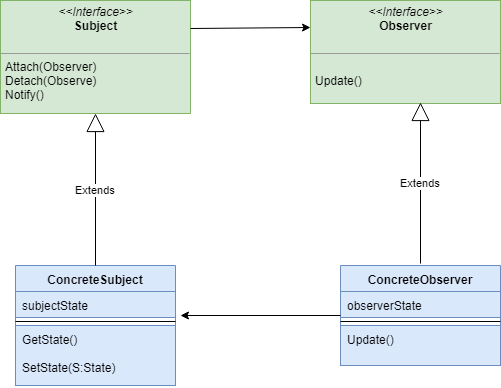
\includegraphics[scale=0.6]{images/observer}
\caption{Struttura observer\label{fig:UC3}}
\end{figure}
\begin{itemize}
	\item \textbf{Subject}
	\begin{itemize}
		\item Il Subject è l'oggetto che notifica li observers;
		\item Il Subject conosce i suoi Observer perchè possiede un riferimento ad essi;
		\item Il metodo \textit{Attach()} serve a sottoscrivere un nuovo observer;
		\item Il metodo \textit{Detach()} serve ad eliminare un observer;
		\item Il metodo \textit{Notify()} sarà implementato dagli observers.
	\end{itemize}
	\item \textbf{ConcreteSubject}
	\begin{itemize}
		\item Quando ConcreteSubject cambia Stato, avverte tutti i ConcreteObserver, attraverso l'invocazione del metodo \textit{Notify()}, ereditato da Subject;
	\end{itemize}
		\item \textbf{Observer}
	\begin{itemize}
		\item Il metodo \textit{Update()} dev'essere implementato dai ConcreteObservers;
	\end{itemize}
	\item \textbf{ConcreteObserver}
	\begin{itemize}
		\item Implementa il metodo \textit{Update()} di Observer;
	\end{itemize}
\end{itemize}

\subsection{Esempio 1}

 Modifica di una o più aree di finestre in risposta alla pressione di un pulsante
\begin{figure}[H]
\centering
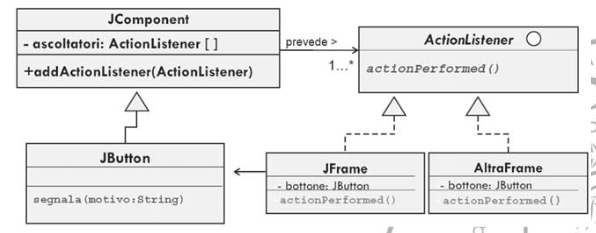
\includegraphics[scale=0.8]{images/esempio1Observer}
\caption{Struttura observer\label{fig:UC3}}
\end{figure}
\begin{itemize}
	\item \textbf{JComponent} agisce da Subject;
	\item \textbf{ActionListener} agisce da Observer;
	\item \textbf{JButton} rappresenta il concreteObserver. È colui che fa scaturire la notifica;
	\item \textbf{JFrame e Altra Frame} rappresentano i concreteObserver;
	\item i 2 concreteObserver hanno un riferimento al concreteSubject ed implementano il metodo \textit{actionPerformed} ereditato da ActionListener;
	\end{itemize}
\section{Proxy}
\subsection{Descrizione}
Si tratta di un pattern strutturale basato su oggetti che viene utilizzato per accedere ad un’oggetto complesso tramite un oggetto semplice.
Questo pattern può risultare utile se l’oggetto complesso:
\begin{itemize}
\item richiede molte risorse computazionali;
\item richiede molto tempo per caricarsi;
\item è presente su una macchina remota e il traffico di rete determina latenze ed overhead;
\item non definisce delle policy di sicurezze e consente un accesso indiscriminato;
\item non viene mantenuto in cache ma viene rigenerato ad ogni richiesta.
\end{itemize}

\subsection{Applicabilità}
\begin{itemize}
	\item \textbf{Remote Proxy}: rappresentazione locale di un oggetto che si trova in uno spazio di indirizzi differenti. Tipicamente permette di accedere a risorse distribuite sulla rete come se fossero accessibili come oggetto locale;
	\item \textbf{Virtual Proxy}: gestisce la creazione su richiesta di oggetti costosi;
	\item \textbf{Protection Proxy}: controlla l'accesso all'oggetto originale. Questo tipo di proxy si rivela utile quando possono essere definiti diritti di accesso diversi per gli oggetti;
	\item \textbf{Riferimento intelligente}: sostituisce un puntatore puro a un oggetto consentendo l'esecuzione di attività aggiunte quando si accede all'oggetto referenzito;
\end{itemize}

\subsection{Struttura}
\begin{figure}[H]
\centering
\includegraphics[scale=0.6]{images/proxy1}
\caption{Struttura proxy\label{fig:UC3}}
\end{figure}


\begin{itemize}
	\item \textbf{Subject}
	\begin{itemize}
		\item La classe Subject è una classe astratta ed è la classe base del Proxy e del RealSubject;
		\item Definisce i membri che verrano implementati dalle sottoclassi;
	\end{itemize}
	\item \textbf{RealSubject}
	\begin{itemize}
		\item La classe RealSubject è la classe complessa che desideriamo utilizzare in modo efficiente, senza tanto sprecco di risorse;
	\end{itemize}
		\item \textbf{Proxy}
	\begin{itemize}
		\item Gli oggetti Proxy contengono un'istanza privata di un oggetto RealSubject;
		\item Gli oggetti Client eseguono azioni sul proxy che vengono passati all'oggetto RealSubject;
		\item I riusltati dei membri di RealSubject vengono restituiti al client tramite il Proxy.
	\end{itemize}
	
\end{itemize}

Nel diagramma delle classi vediamo come il client dipende solamente dall'interfaccia. Invece dell'oggetto reale, il client potrebbe utilizzare il proxy. Quando l'oggetto proxy viene chiamato fa le sue cose e infine inoltra la chiamata all'oggetto reale.

\subsection{Parole chiavi}
\begin{itemize}
\item \textit{remote proxy}: ambasciatore, governare, remoto, oggetti dislocati nella rete;
\item \textit{virtual proxy}: risorse, locale;
\item \textit{puntatore intelligente}: riferimento, locale;
\end{itemize}

\subsection{Associazione}
\begin{itemize}
\item viene spesso associato con un pattern proxy o adapter o strategy;
\end{itemize}



\end{document}
